% Provenance (never printed): see sources/outline_sources.md (Year 2: humidity variables;
% Clausius--Clapeyron applied; dry and moist adiabats; thermodynamic diagrams; convective
% instability; cloud microphysics). Definitions after the NWS glossary; skew-T lines, CAPE classes
% and the lifted index after the NWS Houston/Galveston training page; saturation data from the
% NIST WebBook (IAPWS-95) and IAPWS R14-08; the empirical formula as used by Su and others
% (2026); kappa-Koehler theory after Petters and Kreidenweis (2007); CCN numbers after Andreae
% (2009); the processes of microphysics after Morrison and others (2020). The sounding is the
% real 12 UTC sounding of Norman, Oklahoma, 16 April 2026 (IGRA2); every curve and number from
% figdata/bachelor-2/thermo.py; exercise and problem values in the Book 4 scratch calculator
% calc/ch21.py.
\chapter{Termodinâmica da atmosfera}\label{ch:b2:atmospheric-thermodynamics}

Em 16 de abril de 2026, às 12 UTC, um balão subiu da estação meteorológica de Norman, Oklahoma, como
sobem balões de mais de oitocentas estações a essa hora todos os dias. O instrumento que ele
levava transmitiu por rádio um perfil vertical que um meteorologista lê de relance: ar junto ao solo
quase saturado, uma fina tampa quente a seiscentos metros de altura e, acima dela, uma temperatura que caía
depressa ao longo de dez quilômetros. Levantado através da tampa, o ar da superfície teria se encontrado
mais quente que o ambiente em quase toda a troposfera, com uns dois mil joules por
quilograma para gastar na subida. Este capítulo aprende a ler essa energia numa sondagem: quanta
água o ar contém, como uma parcela que sobe se resfria antes e depois de condensar, como os diagramas dos
meteorologistas transformam áreas em energias, e como as gotículas de nuvem chegam a se formar.
% ledger: data:b4-sounding, nws4:upperair, nws4:cape

\begin{recall}
\textbf{Dos livros de física}: a \omterm{def:b2:atmospheric-thermodynamics:moist-air}{pressão de vapor} de saturação, a umidade relativa, o ponto de orvalho,
o calor latente, a relação de Clausius--Clapeyron e sua forma integrada; a nucleação e o
sobrerresfriamento; a primeira lei, as transformações adiabáticas e as capacidades térmicas de um gás ideal.
\textbf{Dos livros de química}: as pressões parciais, a lei de Raoult, a tensão superficial e a equação
de Kelvin. \textbf{Dos volumes escolares}: o \omterm{def:b2:atmospheric-thermodynamics:lcl}{nível de condensação} e sua regra de
\qty{125}{m} por grau, o ar estável e instável, o \omterm{def:b2:atmospheric-thermodynamics:microphysics}{núcleo de condensação}, os processos de chuva quente e
dos cristais de gelo. \textbf{Do volume do primeiro ano}: a atmosfera padrão, os gradientes térmicos
ambiental e adiabático seco ($\Gamma_d = \qty{9.8}{K/km}$), a parcela de ar, a temperatura
potencial, a estabilidade estática, as inversões térmicas e a equação hipsométrica.
\end{recall}

Ao longo de todo o capítulo: $R_d = R/M_d = \qty{287.0}{J.kg^{-1}.K^{-1}}$ para o ar seco de massa molar
\qty{28.97}{g/mol}; $R_v = R/M_w = \qty{461.5}{J.kg^{-1}.K^{-1}}$ para o vapor de água, de massa
molar \qty{18.0153}{g/mol}; $\varepsilon = M_w/M_d = 0.622$; $c_p = \tfrac72 R_d =
\qty{1004.5}{J.kg^{-1}.K^{-1}}$ (o volume do primeiro ano, com a razão das capacidades térmicas 1.4);
$g = \qty{9.81}{m.s^{-2}}$; e o calor latente de vaporização no ponto triplo,
$L = \qty{2.501e6}{J/kg}$.
% ledger: const:R, earth:Mmol, nist4:water-mw, nasa:grc-gamma, const:gn, nist4:water-sat

\section{O ar úmido}\label{sec:b2:atmospheric-thermodynamics:moist-air}

O ar é uma mistura de ar seco e vapor de água, ambos próximos de gases ideais. Os livros de física
medem sua água pela umidade relativa e pelo ponto de orvalho; uma parcela que sobe precisa de medidas
que não mudem quando ela se expande.

\begin{definition}[Pressão de vapor; razão de mistura; umidade específica]\label{def:b2:atmospheric-thermodynamics:moist-air}
A \emph{pressão de vapor}\index{pressão de vapor} $e$ do ar úmido é a pressão parcial de
seu vapor de água. Sua \emph{razão de mistura}\index{razão de mistura} é $r = m_v/m_d$, a massa de vapor
de água por unidade de massa de ar seco no mesmo volume, e sua \emph{umidade
específica}\index{umidade específica} é $q = m_v/(m_d + m_v)$, a massa de vapor por unidade de massa de
ar úmido. Ambas são dadas em geral em gramas por quilograma.
\end{definition}
% ledger: nws4:humidity

\begin{proposition}[Variáveis de umidade]\label{prop:b2:atmospheric-thermodynamics:humidity}
Num ar úmido à pressão total $p$ com a \omterm{def:b2:atmospheric-thermodynamics:moist-air}{pressão de vapor} $e$,
\[
  r = \frac{\varepsilon e}{p - e}, \qquad q = \frac{r}{1 + r} = \frac{\varepsilon e}{p - (1 -
  \varepsilon)e} .
\]
Na saturação, $e = e_s(T)$ e $r = r_s(T, p)$, a \omterm{def:b2:atmospheric-thermodynamics:moist-air}{razão de mistura} de saturação. Nem $r$ nem
$q$ mudam quando uma parcela se expande ou é comprimida sem ganhar nem perder água.
\end{proposition}

\begin{proof}
No mesmo volume $V$ à temperatura $T$, cada gás obedece à sua própria lei dos gases ideais com sua
pressão parcial: $m_v = eV/(R_vT)$ e $m_d = (p - e)V/(R_dT)$, de modo que $r = (R_d/R_v)\,e/(p - e)$,
e $R_d/R_v = M_w/M_d = \varepsilon$. Dividindo $m_v$ por $m_d + m_v$ obtém-se $q = r/(1 + r)$.
A expansão muda $V$, $p$ e $e$, mas não as duas massas.
\end{proof}

\begin{definition}[Temperatura virtual]\label{def:b2:atmospheric-thermodynamics:virtual}
A \emph{temperatura virtual}\index{temperatura virtual} $T_v$ do ar úmido é a temperatura
que o ar seco precisaria ter, à mesma pressão, para ter a mesma densidade:
\[
  T_v = T\,\frac{1 + r/\varepsilon}{1 + r} \approx T\,(1 + 0.61\,r) .
\]
\end{definition}
% ledger: nws4:virtual-theta-e

A prova de que essa temperatura faz o que diz cabe numa linha: a densidade do ar úmido é
$(m_d + m_v)/V = \bigl(p - e\bigr)/(R_dT) + e/(R_vT)$, que, com $e = pr/(\varepsilon + r)$,
é igual a $p/(R_dT_v)$. O vapor de água é mais leve que o ar seco, de modo que o ar úmido é menos denso que o ar seco
à mesma temperatura e pressão, como se fosse um pouco mais quente.

\begin{example}[O ar de Norman]\label{ex:b2:atmospheric-thermodynamics:norman}
No solo a sondagem dá $p = \qty{971.1}{hPa}$, $T = \qty{19.0}{\celsius}$ e um ponto de orvalho
de \qty{18.5}{\celsius}. A \omterm{def:b2:atmospheric-thermodynamics:moist-air}{pressão de vapor} é a \omterm{def:b2:atmospheric-thermodynamics:moist-air}{pressão de vapor} de saturação no ponto de
orvalho, $e = e_s(\qty{18.5}{\celsius}) = \qty{21.5}{hPa}$ (\cref{prop:b2:atmospheric-thermodynamics:es}
adiante). Então $r = 0.622 \times 21.5/(971.1 - 21.5) = \qty{14.1}{g/kg}$, $q = \qty{13.9}{g/kg}$,
e $T_v - T = 0.61 \times 0.0141 \times \qty{292.15}{K} = \qty{2.5}{K}$: este ar é tão leve quanto
um ar seco dois graus e meio mais quente.
\end{example}
% ledger: data:b4-sounding

\section{A pressão de vapor de saturação}\label{sec:b2:atmospheric-thermodynamics:saturation}

Sobre uma superfície plana de água pura, a \omterm{def:b2:atmospheric-thermodynamics:moist-air}{pressão de vapor} de equilíbrio depende apenas da
temperatura. Os livros de física deduzem sua lei, a relação de Clausius--Clapeyron, e a integram
com um calor latente constante; para o vapor de água, $M L/R = L/R_v$.

\begin{proposition}[Pressão de vapor de saturação]\label{prop:b2:atmospheric-thermodynamics:es}
Com o calor latente $L$ mantido constante, a \omterm{def:b2:atmospheric-thermodynamics:moist-air}{pressão de vapor} de saturação sobre a água é
\[
  e_s(T) = e_t \exp\!\Bigl[\frac{L}{R_v}\Bigl(\frac{1}{T_t} - \frac{1}{T}\Bigr)\Bigr],
  \qquad e_t = \qty{6.117}{hPa}, \quad T_t = \qty{273.16}{K}, \quad \frac{L}{R_v} =
  \qty{5419}{K},
\]
onde $(T_t, e_t)$ é o ponto triplo da água.
\end{proposition}
% ledger: iapws4:sublimation, nist4:water-sat

\begin{corollary}[Sete por cento por kelvin]\label{cor:b2:atmospheric-thermodynamics:seven}
A taxa relativa de aumento da \omterm{def:b2:atmospheric-thermodynamics:moist-air}{pressão de vapor} de saturação é
$\mathrm{d}\ln e_s/\mathrm{d}T = L/(R_v T^2)$: \qty{7.3}{\percent} por kelvin a
\qty{0}{\celsius}, \qty{6.3}{\percent} a \qty{20}{\celsius}, \qty{5.9}{\percent} a
\qty{30}{\celsius}.
\end{corollary}

O calor latente constante é o único defeito da fórmula: o calor latente cai de
\qty{2500.9}{kJ/kg} no ponto triplo para \qty{2453.5}{kJ/kg} a \qty{20}{\celsius}, de modo que a
fórmula se adianta aos valores medidos à medida que a temperatura sobe, em \qty{1.2}{\percent} a
\qty{20}{\celsius} e \qty{2.5}{\percent} a \qty{30}{\celsius} (figura abaixo). Uma fórmula
empírica ajustada às medidas, $e_s = \qty{6.112}{hPa} \times \exp[17.67\,t/(t + 243.5)]$ com
$t$ em graus Celsius, fica dentro de algumas partes por mil; os produtos de dados a usam, mas a
proposição é a que se pode derivar e compreender, e este capítulo a mantém.
% ledger: nist4:water-sat, su26:svp

Abaixo de \qty{0}{\celsius}, a água pode permanecer líquida nas nuvens, sobrerresfriada, e existem duas \omterm{def:b2:atmospheric-thermodynamics:moist-air}{pressões
de vapor} de saturação: sobre a água líquida e sobre o gelo. A segunda é menor, porque o calor latente
de sublimação excede o de vaporização pelo calor latente de fusão. Um ar saturado em
relação a gotículas sobrerresfriadas está supersaturado em relação ao gelo, em \qty{10}{\percent} a
\qty{-10}{\celsius} e \qty{22}{\percent} a \qty{-20}{\celsius}: a última seção volta a
essa diferença.
% ledger: iapws4:sublimation, su26:svp

\begin{omfigure}
\centering
% figdata/bachelor-2/thermo.py parts es, nist
\begin{tikzpicture}
\begin{groupplot}[group style={group size=2 by 1, horizontal sep=1.9cm},
  width=0.44\linewidth, height=5.4cm, tick label style={font=\scriptsize},
  label style={font=\small}]
\nextgroupplot[xmin=-40, xmax=40, ymin=0, ymax=80, xlabel={temperatura (\unit{\celsius})},
  ylabel={pressão de vapor de saturação (\unit{hPa})}, legend pos=north west,
  legend style={font=\scriptsize, draw=none, fill=none}, legend cell align=left]
\addplot[ocBlue, thick] table[x=T_C, y=cc] {figdata/out/bachelor-2-thermo-es.dat};
\addlegendentry{proposição}
\addplot[black, densely dashed] table[x=T_C, y=emp] {figdata/out/bachelor-2-thermo-es.dat};
\addlegendentry{fórmula empírica}
\addplot[only marks, mark=*, mark size=1.4pt, ocRed] table[x=T_C, y=es_hPa]
  {figdata/out/bachelor-2-thermo-nist.dat};
\addlegendentry{medida (IAPWS-95)}
\nextgroupplot[xmin=-40, xmax=0, ymin=1, ymax=1.5, xlabel={temperatura (\unit{\celsius})},
  ylabel={$e_s(\text{água})/e_s(\text{gelo})$}]
\addplot[omMeth, thick, unbounded coords=discard] table[x=T_C, y=wi]
  {figdata/out/bachelor-2-thermo-es.dat};
\draw[black!40, densely dotted] (axis cs:-10,1) -- (axis cs:-10,1.1035) -- (axis cs:-40,1.1035);
\node[font=\scriptsize, anchor=south west] at (axis cs:-10,1.1035) {1.10};
\draw[black!40, densely dotted] (axis cs:-20,1) -- (axis cs:-20,1.218) -- (axis cs:-40,1.218);
\node[font=\scriptsize, anchor=south west] at (axis cs:-20,1.218) {1.22};
\end{groupplot}
\end{tikzpicture}
\par\smallskip{\small Esquerda: a \omterm{def:b2:atmospheric-thermodynamics:moist-air}{pressão de vapor} de saturação sobre a água pela
\cref{prop:b2:atmospheric-thermodynamics:es}, pela fórmula empírica e tal como medida. Direita: a
razão entre as \omterm{def:b2:atmospheric-thermodynamics:moist-air}{pressões de vapor} de saturação sobre a água sobrerresfriada (fórmula empírica) e sobre o gelo
(equação de sublimação da IAPWS).}
\end{omfigure}
% ledger: nist4:water-sat, iapws4:sublimation, su26:svp

\section{O ar úmido que sobe}\label{sec:b2:atmospheric-thermodynamics:ascent}

Uma parcela que sobe sem trocar calor resfria-se segundo o gradiente adiabático seco, conserva sua
temperatura potencial e, se não condensa, conserva sua \omterm{def:b2:atmospheric-thermodynamics:moist-air}{razão de mistura}. Sua \omterm{def:b2:atmospheric-thermodynamics:moist-air}{pressão de vapor}
$e = pr/(\varepsilon + r)$ cai com a pressão, mas sua \omterm{def:b2:atmospheric-thermodynamics:moist-air}{pressão de vapor} de saturação cai
mais depressa, com sua temperatura. As duas se encontram num nível que os volumes escolares obtinham por uma regra.

\begin{definition}[Nível de condensação por levantamento]\label{def:b2:atmospheric-thermodynamics:lcl}
O \emph{nível de condensação por levantamento}\index{nível de condensação por levantamento} (NCL) de uma parcela é o
nível em que ela se torna saturada quando é levantada adiabaticamente a seco. É o
\emph{nível de condensação}\index{nível de condensação} dos volumes escolares, a altura das
bases planas das nuvens que se formam por levantamento.
\end{definition}
% ledger: nws4:lcl

\begin{proposition}[Altura do nível de condensação por levantamento]\label{prop:b2:atmospheric-thermodynamics:lcl}
Uma parcela à temperatura $T$ com o ponto de orvalho $T_d$ atinge a saturação a cerca de
\[
  z_{\text{NCL}} \approx \frac{T - T_d}{\Gamma_d - \Gamma_{\text{orv}}}, \qquad
  \Gamma_{\text{orv}} = \frac{g R_v T_d^2}{L R_d T} \approx \qty{1.8}{K/km},
\]
acima de seu nível de partida: cerca de \qty{125}{m} para cada grau de depressão do ponto de orvalho.
\end{proposition}

\begin{proof}
A temperatura da parcela cai segundo $\Gamma_d$. Seu ponto de orvalho é a temperatura na qual sua
\omterm{def:b2:atmospheric-thermodynamics:moist-air}{pressão de vapor} $e$ saturaria; com $r$ constante, $e$ é proporcional a $p$, de modo que
$\mathrm{d}\ln e = \mathrm{d}\ln p = -g\,\mathrm{d}z/(R_dT)$ pelo equilíbrio hidrostático. Pela
\cref{prop:b2:atmospheric-thermodynamics:es}, $\mathrm{d}\ln e = L\,\mathrm{d}T_d/(R_vT_d^2)$.
Daí $\mathrm{d}T_d/\mathrm{d}z = -gR_vT_d^2/(LR_dT) = -\Gamma_{\text{orv}}$: o ponto de orvalho também cai,
mas mais devagar. A diferença $T - T_d$ fecha-se à taxa $\Gamma_d - \Gamma_{\text{orv}}$. Com
$T \approx T_d \approx \qty{288}{K}$, $\Gamma_{\text{orv}} = \qty{1.8}{K/km}$, e $1/(9.8 - 1.8)$
quilômetros por kelvin são \qty{125}{m}.
\end{proof}

Em Norman a depressão do ponto de orvalho era de \qty{0.5}{K}: o ar da superfície teria condensado depois de
\qty{63}{m} de subida, a \qty{964}{hPa}. O cálculo completo, que segue a adiabática seca e
a \omterm{def:b2:atmospheric-thermodynamics:moist-air}{razão de mistura} de saturação sem linearizar, dá \qty{64}{m}.
% ledger: data:b4-sounding

Acima do NCL a parcela condensa à medida que sobe. A condensação libera calor latente, e a parcela
resfria-se mais devagar.

\begin{definition}[Gradiente adiabático saturado; adiabática úmida]\label{def:b2:atmospheric-thermodynamics:moist-adiabat}
O \emph{gradiente adiabático saturado}\index{gradiente adiabático saturado} $\Gamma_s$ é
a taxa à qual a temperatura de uma parcela saturada cai à medida que ela sobe, com seu vapor condensando
para mantê-la saturada. A curva que ela segue num diagrama de temperatura em função da pressão é uma
\emph{adiabática úmida}\index{adiabática úmida}. Quando se supõe que a água condensada cai
imediatamente, a subida é chamada pseudoadiabática.
\end{definition}
% ledger: nws4:malr

\begin{proposition}[Gradiente adiabático saturado]\label{prop:b2:atmospheric-thermodynamics:gamma-s}
Para uma subida pseudoadiabática, com $r_s = r_s(T, p)$,
\[
  \Gamma_s = g\,\frac{1 + \dfrac{L r_s}{R_d T}}{c_p + \dfrac{L^2 r_s}{R_v T^2}} .
\]
Ele tende a $\Gamma_d = g/c_p$ quando $r_s$ tende a zero, e é menor nos outros casos.
\end{proposition}

\begin{proof}
Por unidade de massa de ar seco, a primeira lei para uma parcela que recebe o calor latente do vapor
que condensa, $-L\,\mathrm{d}r_s$, escreve-se $c_p\,\mathrm{d}T - (R_dT/p)\,\mathrm{d}p = -L\,
\mathrm{d}r_s$; com o equilíbrio hidrostático $(R_dT/p)\,\mathrm{d}p = -g\,\mathrm{d}z$, ela se torna
$c_p\,\mathrm{d}T + g\,\mathrm{d}z + L\,\mathrm{d}r_s = 0$. Com $r_s \approx \varepsilon e_s/p$,
$\mathrm{d}r_s = r_s\,(\mathrm{d}\ln e_s - \mathrm{d}\ln p) = r_s\bigl(L\,\mathrm{d}T/(R_vT^2) +
g\,\mathrm{d}z/(R_dT)\bigr)$. Substituindo e agrupando os termos em $\mathrm{d}T$ e em
$\mathrm{d}z$ obtém-se $-\mathrm{d}T/\mathrm{d}z = \Gamma_s$.
\end{proof}

O gradiente depende de quanta água há para condensar. A \qty{1000}{hPa} ele vale
\qty{6.5}{K/km} a \qty{0}{\celsius}, \qty{5.2}{K/km} a \qty{10}{\celsius}, \qty{4.2}{K/km} a
\qty{20}{\celsius} e \qty{3.4}{K/km} a \qty{30}{\celsius}; no alto da troposfera, a
\qty{200}{hPa} e \qty{-60}{\celsius}, volta a \qty{9.6}{K/km}, quase o gradiente seco. Uma
\omterm{def:b2:atmospheric-thermodynamics:moist-adiabat}{adiabática úmida} é, portanto, íngreme perto do solo quente e se inclina para as adiabáticas secas em altitude.
% ledger: nws4:malr

\begin{definition}[Temperatura potencial equivalente]\label{def:b2:atmospheric-thermodynamics:theta-e}
A \emph{temperatura potencial equivalente}\index{temperatura potencial equivalente} $\theta_e$ de
uma parcela é a temperatura que ela teria se fosse levantada até que todo o seu vapor tivesse condensado
e caído, e depois trazida de volta adiabaticamente a seco até \qty{1000}{hPa}. Uma boa aproximação é
\[
  \theta_e \approx \theta \exp\!\Bigl(\frac{L r}{c_p T_{\text{NCL}}}\Bigr),
\]
sendo $\theta$ a temperatura potencial e $T_{\text{NCL}}$ a temperatura no \omterm{def:b2:atmospheric-thermodynamics:lcl}{nível de
condensação por levantamento} da parcela.
\end{definition}
% ledger: nws4:virtual-theta-e

A temperatura potencial só se conserva na subida seca; $\theta_e$ conserva-se, nesta
aproximação, tanto na subida seca quanto na saturada, porque o calor que ela conta como já liberado
é exatamente o calor que a condensação libera. Ela rotula uma \omterm{def:b2:atmospheric-thermodynamics:moist-adiabat}{adiabática úmida} como $\theta$ rotula uma seca.
O ar da superfície de Norman tem $\theta = 292.15 \times (1000/971.1)^{2/7} = \qty{294.6}{K}$ e
$\theta_e = 294.6 \exp[2.501 \times 10^6 \times 0.0141/(1004.5 \times 291.5)] = \qty{332}{K}$.
% ledger: data:b4-sounding

\section{Diagramas termodinâmicos}\label{sec:b2:atmospheric-thermodynamics:diagrams}

\begin{definition}[Sondagem atmosférica]\label{def:b2:atmospheric-thermodynamics:sounding}
Uma \emph{sondagem atmosférica}\index{sondagem atmosférica} é um perfil vertical da
pressão, da temperatura, da umidade e do vento da atmosfera acima de um lugar, medido por um
instrumento levado ao alto, geralmente uma radiossonda sob um balão.
\end{definition}
% ledger: nws:radiosonde, nws4:upperair

Uma sondagem não é bem vertical, porque o balão deriva com o vento, nem bem
instantânea, porque leva vários minutos para chegar à alta troposfera; e a rede principal
só faz lançamentos duas vezes por dia. Seus números tornam-se úteis quando traçados num diagrama
em que uma parcela que sobe pode ser acompanhada com uma régua.
% ledger: hgx:skewt-lines

\begin{definition}[Diagrama termodinâmico; diagrama skew-T log-p; tefigrama]\label{def:b2:atmospheric-thermodynamics:diagram}
Um \emph{diagrama termodinâmico}\index{diagrama termodinâmico} é um gráfico cujas coordenadas são
funções da pressão e da temperatura, no qual estão impressas isóbaras, isotermas, adiabáticas secas, \omterm{def:b2:atmospheric-thermodynamics:moist-adiabat}{adiabáticas
úmidas} e linhas de \omterm{def:b2:atmospheric-thermodynamics:moist-air}{razão de mistura} de saturação constante, e no qual uma sondagem é
traçada como duas curvas, sua temperatura e seu ponto de orvalho. Num \emph{diagrama skew-T
log-p}\index{diagrama skew-T log-p} a coordenada vertical é $-\ln p$ e a horizontal é
$T + k\ln(p_0/p)$, de modo que as isóbaras são horizontais e as isotermas são retas inclinadas subindo para
a direita. Um \emph{tefigrama}\index{tefigrama} usa como coordenadas a temperatura e a entropia por unidade de
massa $c_p\ln\theta$, de modo que as isotermas e as adiabáticas secas são retas
perpendiculares.
\end{definition}
% ledger: hgx:skewt-lines

\begin{proposition}[As áreas são energias]\label{prop:b2:atmospheric-thermodynamics:areas}
Num \omterm{def:b2:atmospheric-thermodynamics:diagram}{diagrama skew-T log-p}, a área compreendida entre duas curvas $T_1(p)$ e $T_2(p)$ entre as
pressões $p_b > p_a$ é proporcional a $\int_{p_a}^{p_b} R_d\,(T_1 - T_2)\,\mathrm{d}\ln p$,
a energia por unidade de massa que a \cref{prop:b2:atmospheric-thermodynamics:buoyancy} adiante dá a
uma parcela que segue $T_1$ através de um ambiente $T_2$.
\end{proposition}

\begin{proof}
Tome-se $Y = \ln(p_0/p)$ e $X = T + kY$. O jacobiano de $(T, Y) \mapsto (X, Y)$ é 1, de modo que as áreas no
plano $(X, Y)$ são iguais às áreas no plano $(T, Y)$, onde a área entre duas curvas é
$\int (T_1 - T_2)\,\mathrm{d}Y = \int (T_1 - T_2)\,\mathrm{d}\ln p$ tomada de $p_a$ a $p_b$
com o sinal fixado. Multiplicando por $R_d$ e pela escala do diagrama obtém-se a energia.
\end{proof}

\begin{method}[Levantar uma parcela num diagrama]\label{met:b2:atmospheric-thermodynamics:lift}
\begin{enumerate}
  \item Trace a temperatura e o ponto de orvalho da sondagem em função da pressão.
  \item A partir da temperatura da parcela, siga a adiabática seca para cima; a partir de seu ponto de orvalho, siga
        a linha de \omterm{def:b2:atmospheric-thermodynamics:moist-air}{razão de mistura} de saturação. Onde elas se encontram fica o NCL.
  \item A partir do NCL, siga a \omterm{def:b2:atmospheric-thermodynamics:moist-adiabat}{adiabática úmida} para cima.
  \item Onde a curva da parcela fica à direita da temperatura da sondagem, a parcela está
        mais quente que o ambiente; os níveis onde as duas curvas se cruzam são os níveis da
        \cref{def:b2:atmospheric-thermodynamics:parcel-levels} adiante.
\end{enumerate}
\end{method}
% ledger: hgx:skewt-lines


\section{Estabilidade e energia convectiva}\label{sec:b2:atmospheric-thermodynamics:stability}

O volume do primeiro ano comparou o gradiente $\Gamma$ de uma camada com $\Gamma_d$. Uma parcela saturada
resfria-se segundo $\Gamma_s$, e um terceiro caso aparece entre os dois gradientes.

\begin{definition}[Instabilidade condicional]\label{def:b2:atmospheric-thermodynamics:instability}
Uma camada cujo gradiente fica entre o \omterm{def:b2:atmospheric-thermodynamics:moist-adiabat}{gradiente adiabático saturado} e o seco,
$\Gamma_s < \Gamma < \Gamma_d$, está em \emph{instabilidade condicional}\index{instabilidade condicional}:
estável para as parcelas não saturadas, instável para as saturadas.
\end{definition}
% ledger: nws4:malr

Em Norman a temperatura caiu \qty{37.0}{K} entre \qty{850}{hPa} (\qty{1489}{m}) e
\qty{500}{hPa} (\qty{5725}{m}), a \qty{8.7}{K/km}: \omterm{def:b2:atmospheric-thermodynamics:instability}{instabilidade condicional} ao longo de quatro quilômetros.
Se a instabilidade é liberada depende de onde uma parcela vinda de baixo se torna saturada e
depois mais quente que o ambiente.
% ledger: data:b4-sounding

\begin{definition}[Nível de convecção espontânea; nível de equilíbrio]\label{def:b2:atmospheric-thermodynamics:parcel-levels}
O \emph{nível de convecção espontânea}\index{nível de convecção espontânea} (NCE) de uma parcela levantada é
o nível acima do qual, saturada, ela se torna mais quente que o ambiente e sobe livremente. O
\emph{nível de equilíbrio}\index{nível de equilíbrio} (NE) é o nível acima do NCE em que sua
temperatura volta a igualar a do ambiente.
\end{definition}
% ledger: nws4:lfc-el

\begin{omfigure}
\centering
% figdata/bachelor-2/thermo.py parts iso, dry, moist, mix, env, dew, parcel, cape, cin, marks
\begin{tikzpicture}
\begin{axis}[width=0.86\linewidth, height=10.6cm, ymode=log, y dir=reverse, ymin=100,
  ymax=1050, xmin=-42, xmax=44, clip=true,
  ytick={100,200,300,400,500,700,850,1000}, yticklabels={100,200,300,400,500,700,850,1000},
  minor ytick={}, xtick={-41.464,-31.464,-21.464,-11.464,-1.464,8.536,18.536,28.536,38.536},
  xticklabels={$-40$,$-30$,$-20$,$-10$,0,10,20,30,40}, tick label style={font=\scriptsize},
  xlabel={temperatura (\unit{\celsius}), lida ao longo das isotermas inclinadas},
  ylabel={pressão (\unit{hPa})}, label style={font=\small},
  legend style={font=\scriptsize, at={(0.985,0.985)}, anchor=north east, fill=white,
  fill opacity=0.9, text opacity=1, draw=black!30}, legend cell align=left]
\addplot[fill=ocRed, fill opacity=0.28, draw=none, forget plot] table[x=x, y=p]
  {figdata/out/bachelor-2-thermo-cape.dat};
\addplot[fill=ocBlue, fill opacity=0.28, draw=none, forget plot] table[x=x, y=p]
  {figdata/out/bachelor-2-thermo-cin.dat};
\addplot[black!22, very thin, forget plot] table[x=x, y=p] {figdata/out/bachelor-2-thermo-iso.dat};
\addplot[orange!70!black, very thin, opacity=0.55] table[x=x, y=p]
  {figdata/out/bachelor-2-thermo-dry.dat};
\addlegendentry{adiabáticas secas}
\addplot[omMeth, very thin, densely dashed, opacity=0.7] table[x=x, y=p]
  {figdata/out/bachelor-2-thermo-moist.dat};
\addlegendentry{adiabáticas úmidas}
\addplot[ocBlue, thin, dotted] table[x=x, y=p]
  {figdata/out/bachelor-2-thermo-mix.dat};
\addlegendentry{razão de mistura de saturação}
\addplot[ocRed, thick] table[x=x, y=p] {figdata/out/bachelor-2-thermo-env.dat};
\addlegendentry{temperatura}
\addplot[omMeth!70!black, thick] table[x=x, y=p] {figdata/out/bachelor-2-thermo-dew.dat};
\addlegendentry{ponto de orvalho}
\addplot[black, thick, dashed] table[x=x, y=p] {figdata/out/bachelor-2-thermo-parcel.dat};
\addlegendentry{parcela da superfície}
\foreach \r/\x in {1/-7.948, 2/0.283, 4/9.053, 8/18.396, 16/28.323} {
  \edef\tmp{\noexpand\node[font=\noexpand\tiny, ocBlue, anchor=south] at (axis cs:\x,600) {\r};}\tmp
}
\addplot[only marks, mark=*, mark size=1.6pt, black, forget plot] table[x=x, y=p]
  {figdata/out/bachelor-2-thermo-marks.dat};
\node[font=\scriptsize, anchor=west] at (axis cs:20.5,963.9) {NCL};
\node[font=\scriptsize, anchor=west] at (axis cs:18.2,732.5) {NCE};
\node[font=\scriptsize, anchor=east] at (axis cs:-9.6,235.6) {NE};
\node[font=\scriptsize, ocRed!70!black] at (axis cs:2,420) {CAPE};
\node[font=\scriptsize, ocBlue!70!black, anchor=west] at (axis cs:27,860) {CIN};
\end{axis}
\end{tikzpicture}
\par\smallskip{\small A sondagem das 12 UTC de Norman, Oklahoma, em 16 de abril de 2026, num \omterm{def:b2:atmospheric-thermodynamics:diagram}{diagrama skew-T
log-p}, com a parcela da superfície levantada ao longo de sua adiabática seca até o NCL e sua \omterm{def:b2:atmospheric-thermodynamics:moist-adiabat}{adiabática
úmida} acima dele. Vermelho: a área positiva (CAPE); azul: a área negativa abaixo do NCE (CIN), ambas
calculadas com a temperatura. Razões de mistura de saturação em gramas por quilograma, indicadas a
\qty{600}{hPa}.}
\end{omfigure}
% ledger: data:b4-sounding, hgx:skewt-lines

\begin{definition}[Energia potencial convectiva disponível; inibição convectiva]\label{def:b2:atmospheric-thermodynamics:cape}
A \emph{energia potencial convectiva disponível}\index{energia potencial convectiva disponível}
(CAPE) de uma parcela é o trabalho da força de empuxo sobre uma unidade de massa dela entre seu NCE e seu
NE,
\[
  \text{CAPE} = \int_{z_{\text{NCE}}}^{z_{\text{NE}}} g\,\frac{T_{v,\text{parcela}} -
  T_{v,\text{amb}}}{T_{v,\text{amb}}}\,\mathrm{d}z ,
\]
e sua \emph{inibição convectiva}\index{inibição convectiva} (CIN) é a mesma integral,
negativa, de seu nível de partida até seu NCE.
\end{definition}
% ledger: nws4:cape, nws4:cin

\begin{proposition}[O empuxo num diagrama; a velocidade da parcela]\label{prop:b2:atmospheric-thermodynamics:buoyancy}
\begin{enumerate}
  \item Em termos de pressão, $\text{CAPE} = R_d \int_{p_{\text{NE}}}^{p_{\text{NCE}}}
        (T_{v,\text{parcela}} - T_{v,\text{amb}})\,\mathrm{d}\ln p$: num \omterm{def:b2:atmospheric-thermodynamics:diagram}{diagrama skew-T log-p}, ela é
        proporcional à área entre a curva da parcela e a sondagem.
  \item Uma parcela que deixa o NCE em repouso e conserva todo o trabalho de seu empuxo chega ao
        NE com a velocidade vertical $w_{\max} = \sqrt{2\,\text{CAPE}}$.
\end{enumerate}
\end{proposition}

\begin{proof}
1. A parcela e o ambiente compartilham a pressão, de modo que a razão das densidades é a razão das
temperaturas virtuais e a força de empuxo por unidade de massa é
$g(T_{v,\text{parcela}} - T_{v,\text{amb}})/T_{v,\text{amb}}$. O ambiente é hidrostático:
$\mathrm{d}z = -R_dT_{v,\text{amb}}\,\mathrm{d}\ln p/g$. A substituição cancela $g$ e
$T_{v,\text{amb}}$; a área decorre da \cref{prop:b2:atmospheric-thermodynamics:areas}.
2. Sendo $b$ a força de empuxo por unidade de massa, $\mathrm{d}w/\mathrm{d}t = b$ e $w = \mathrm{d}z/
\mathrm{d}t$ dão $w\,\mathrm{d}w = b\,\mathrm{d}z$; integrando do NCE, onde $w = 0$, até
o NE obtém-se $w^2/2 = \text{CAPE}$.
\end{proof}

\begin{example}[A energia na sondagem de Norman]\label{ex:b2:atmospheric-thermodynamics:cape}
Levante-se o ar da superfície do \cref{ex:b2:atmospheric-thermodynamics:norman}. Ele se satura a
\qty{964}{hPa}, \qty{64}{m} acima, e segue uma \omterm{def:b2:atmospheric-thermodynamics:moist-adiabat}{adiabática úmida}. Abaixo de \qty{900}{hPa} a sondagem está
ela própria quase saturada e a parcela fica alguns décimos de grau mais fria que o
ambiente; vem então a inversão entre \qty{908}{hPa} e \qty{889}{hPa}, onde a
temperatura sobe \qty{4.1}{K} em \qty{178}{m} e a parcela se vê \qty{5}{K} fria demais.
Ela só fica mais quente que o ambiente a \qty{732}{hPa}, \qty{2.4}{km} acima do
solo, seu NCE, e continua mais quente até seu NE a \qty{236}{hPa}, \qty{10.9}{km} acima do nível do mar,
logo abaixo da tropopausa que a sondagem indica a \qty{235}{hPa}. Numa grade fina de pressões as
áreas da figura skew-T são CAPE $= \qty{2100}{J/kg}$ e CIN $= \qty{-200}{J/kg}$ com a
temperatura, e \qty{2230}{J/kg} e \qty{-130}{J/kg} com a \omterm{def:b2:atmospheric-thermodynamics:virtual}{temperatura virtual}: a umidade
da parcela acrescenta seu próprio empuxo. A teoria da parcela dá $w_{\max} = \sqrt{2 \times 2100} =
\qty{65}{m/s}$.
\end{example}
% ledger: data:b4-sounding

As tabelas dos meteorologistas chamam uma CAPE de até \qty{1500}{J/kg} de positiva, uma entre 1500 e
\qty{2500}{J/kg} de grande e uma acima de \qty{2500}{J/kg} de extrema; valores acima de \qty{1000}{J/kg} são comuns em ambientes de tempestades,
e raros excedem \qty{5000}{J/kg}. A CAPE é maior na estação quente, especialmente no fim da
primavera. O índice de levantamento, a temperatura da sondagem a \qty{500}{hPa} menos a da parcela
levantada, resume a mesma informação num só número: em Norman, $-18.4 - (-8.9) = \qty{-9.5}{K}$,
na classe de $-8$ a $-10$ que as tabelas dos meteorologistas chamam de instabilidade extrema. Nenhum
desses valores é um limiar acima do qual as tempestades têm de se formar.
% ledger: hgx:cape, nws4:cape, nws4:lifted-index

A CIN é o preço da entrada. A tampa quente impedia o ar da superfície de subir por si mesmo: uma
parcela teria de ser empurrada através dela, por uma frente ou pela lenta ascensão do ar à frente de
uma perturbação em altitude, ou aquecida por baixo pelo sol da tarde até ter empuxo em toda a subida.
E a velocidade $w_{\max}$ é um limite superior: uma corrente ascendente real carrega sua água condensada, que
a torna mais pesada, e mistura-se com o ar mais seco à sua volta, que a resfria por evaporação. O
\omterm{def:b2:atmospheric-thermodynamics:parcel-levels}{nível de equilíbrio} continua sendo um bom guia para onde os topos das tempestades se espalham numa bigorna.
% ledger: nws4:cin, hgx:cape, nws4:lfc-el

\begin{omfigure}
\centering
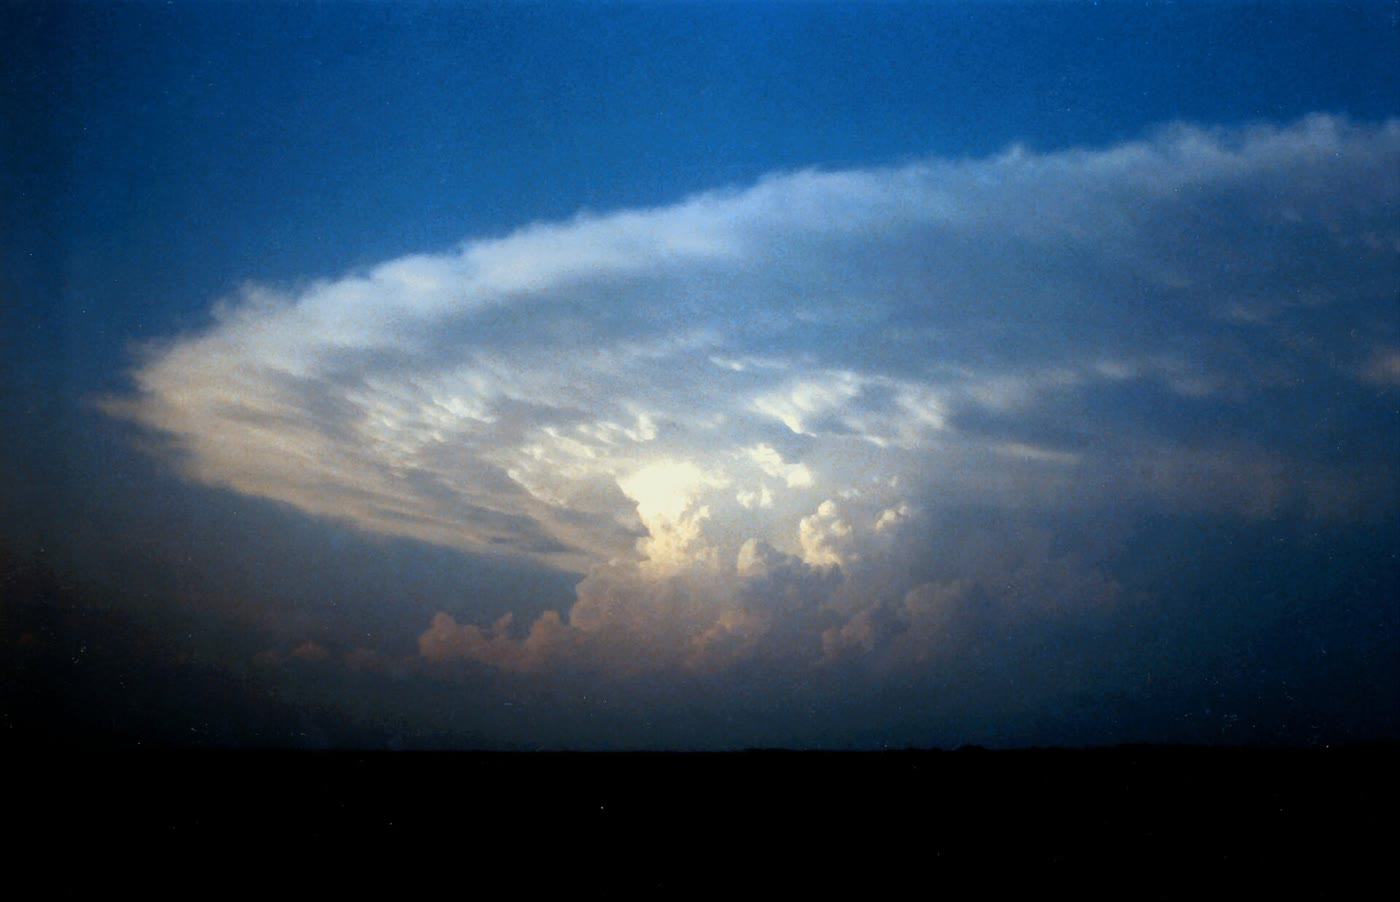
\includegraphics[width=0.6\linewidth]{images/book4/b2-21-supercell-anvil.jpg}
\par\smallskip{\small Uma tempestade sobre o Nebraska, 20 de abril de 1985: sua corrente ascendente se espalha numa
bigorna ao atingir seu \omterm{def:b2:atmospheric-thermodynamics:parcel-levels}{nível de equilíbrio}, perto da tropopausa. (Stephen Corfidi,
NOAA/NWS, domínio público, via Wikimedia Commons.)}
\end{omfigure}
% ledger: nws4:lfc-el

\section{Microfísica das nuvens}\label{sec:b2:atmospheric-thermodynamics:microphysics}

Uma parcela no seu NCL está saturada em relação a uma superfície plana de água. Uma gotícula não é plana: os livros de
física mostram que uma nova fase não aparece no equilíbrio, mas apenas por nucleação, e os
livros de química que a \omterm{def:b2:atmospheric-thermodynamics:moist-air}{pressão de vapor} sobre uma superfície curva excede a pressão sobre uma superfície plana
(a equação de Kelvin). Com a constante $A$ da \cref{prop:b2:atmospheric-thermodynamics:kohler}
adiante, uma gotícula de água pura de \qty{2}{nm} de diâmetro só está em equilíbrio com a razão de saturação
$\exp(2.1/2) = 2.9$, uma \omterm{def:b2:atmospheric-thermodynamics:microphysics}{supersaturação} de \qty{190}{\percent}, muito acima das frações de um por
cento com que as partículas se ativam: as gotículas formam-se sobre partículas.

\begin{definition}[Supersaturação; núcleo de condensação de nuvens]\label{def:b2:atmospheric-thermodynamics:microphysics}
A \emph{supersaturação}\index{supersaturação} do ar é $s = e/e_s - 1$, o excesso de sua
\omterm{def:b2:atmospheric-thermodynamics:moist-air}{pressão de vapor} sobre a \omterm{def:b2:atmospheric-thermodynamics:moist-air}{pressão de vapor} de saturação acima de uma superfície plana de água pura, dado
em geral em porcentagem. Um \emph{núcleo de condensação de nuvens}\index{núcleo de condensação de nuvens} (NCN)
é uma partícula de aerossol sobre a qual uma gotícula de nuvem se forma às pequenas supersaturações das nuvens.
É o \emph{núcleo de condensação}\index{núcleo de condensação} dos volumes escolares.
\end{definition}
% ledger: nws4:ccn-bergeron, pk07:kohler, morrison20:processes

\begin{proposition}[Curva de Köhler]\label{prop:b2:atmospheric-thermodynamics:kohler}
\index{curva de Köhler}
Uma gotícula de solução de diâmetro $D$ crescida sobre uma partícula seca de diâmetro $D_d$ e higroscopicidade
$\kappa$ está em equilíbrio com a razão de saturação
\[
  S(D) = \frac{D^3 - D_d^3}{D^3 - D_d^3(1 - \kappa)}\,\exp\Bigl(\frac{A}{D}\Bigr), \qquad
  A = \frac{4\sigma M_w}{R T\rho_w},
\]
sendo $\sigma$ a tensão superficial e $\rho_w$ a densidade da água (admitido). A curva $S(D)$
é a \emph{\omterm{prop:b2:atmospheric-thermodynamics:kohler}{curva de Köhler}}. Para $D \gg D_d$,
\[
  s = S - 1 \approx \frac{A}{D} - \frac{\kappa D_d^3}{D^3},
\]
que é máxima no diâmetro e na \omterm{def:b2:atmospheric-thermodynamics:microphysics}{supersaturação} críticos
\[
  D_c = \sqrt{\frac{3\kappa D_d^3}{A}}, \qquad s_c = \sqrt{\frac{4A^3}{27\,\kappa D_d^3}} .
\]
\end{proposition}
% ledger: pk07:kohler

\begin{proof}[Demonstração da aproximação]
A exponencial é o fator de Kelvin; a fração é a atividade da água, uma versão da lei de Raoult
na qual $\kappa$ mede quanta água a matéria dissolvida retém. Para $D \gg D_d$ e
$A \ll D$, $\exp(A/D) \approx 1 + A/D$ e a fração é $1 - \kappa D_d^3/D^3$ em primeira
ordem; o produto, em primeira ordem, é $1 + A/D - \kappa D_d^3/D^3$. Anulando a derivada
$-A/D^2 + 3\kappa D_d^3/D^4$ obtém-se $D_c^2 = 3\kappa D_d^3/A$, e então $s_c = A/D_c -
A/(3D_c) = 2A/(3D_c)$, que é a fórmula.
\end{proof}

Com $\sigma = \qty{0.072}{J/m^2}$ a \qty{298.15}{K}, $A = \qty{2.1}{nm}$. O sulfato de amônio tem
$\kappa = 0.61$; o cloreto de sódio é ainda mais higroscópico ($\kappa = 1.28$), e as partículas atmosféricas ficam em geral entre 0.1 e 0.9.
Uma partícula seca de \qty{50}{nm} de sulfato de amônio tem $D_c = \qty{0.33}{\micro m}$ e $s_c =
\qty{0.42}{\percent}$; uma de \qty{100}{nm}, \qty{0.93}{\micro m} e \qty{0.15}{\percent}. A
aproximação difere do máximo exato em menos de \qty{1}{\percent}.
% ledger: pk07:kohler, pk07:kappa

\begin{omfigure}
\centering
% figdata/bachelor-2/thermo.py part kohler
\begin{tikzpicture}
\begin{semilogxaxis}[width=0.72\linewidth, height=5.6cm, xmin=0.03, xmax=10, ymin=-0.4,
  ymax=1.1, xlabel={diâmetro da gotícula $D$ (\unit{\micro m})}, ylabel={supersaturação $s$
  (\unit{\percent})}, tick label style={font=\scriptsize}, label style={font=\small},
  log ticks with fixed point, legend style={font=\scriptsize, draw=none, fill=none},
  legend pos=north east, legend cell align=left, unbounded coords=discard]
\addplot[ocBlue, thick, densely dotted] table[x=D_um, y=s30] {figdata/out/bachelor-2-thermo-kohler.dat};
\addlegendentry{$D_d = \qty{30}{nm}$}
\addplot[ocBlue, thick] table[x=D_um, y=s50] {figdata/out/bachelor-2-thermo-kohler.dat};
\addlegendentry{$D_d = \qty{50}{nm}$}
\addplot[ocBlue, thick, dashed] table[x=D_um, y=s100] {figdata/out/bachelor-2-thermo-kohler.dat};
\addlegendentry{$D_d = \qty{100}{nm}$}
\addplot[only marks, mark=*, mark size=1.5pt, black] coordinates {(0.1542,0.914) (0.3309,0.4244)
  (0.9345,0.1499)};
\draw[black!45] (axis cs:0.03,0) -- (axis cs:10,0);
\draw[ocRed, densely dashed] (axis cs:0.03,0.5) -- (axis cs:10,0.5);
\node[font=\scriptsize, ocRed, anchor=north west] at (axis cs:2.2,0.5) {$s = \qty{0.5}{\percent}$};
\end{semilogxaxis}
\end{tikzpicture}
\par\smallskip{\small \omterm{prop:b2:atmospheric-thermodynamics:kohler}{Curvas de Köhler} de partículas de sulfato de amônio ($\kappa = 0.61$) de três diâmetros
secos a \qty{298.15}{K}, com seus pontos críticos (pontos). Num ar a \qty{0.5}{\percent} de
\omterm{def:b2:atmospheric-thermodynamics:microphysics}{supersaturação}, as partículas de \qty{50}{nm} e de \qty{100}{nm} crescem sem limite; a
partícula de \qty{30}{nm} continua sendo uma gotícula de névoa seca.}
\end{omfigure}
% ledger: pk07:kohler, pk07:kappa

A curva separa as partículas. Abaixo de seu pico uma gotícula está em equilíbrio estável: se cresce,
o ar já não está supersaturado o bastante para ela e ela volta a encolher; essas gotículas de névoa seca incham
e encolhem com a umidade. Quando a \omterm{def:b2:atmospheric-thermodynamics:microphysics}{supersaturação} do ar excede $s_c$, a gotícula é
\emph{ativada}: passado o pico, ela precisa de cada vez menos \omterm{def:b2:atmospheric-thermodynamics:microphysics}{supersaturação} à medida que cresce, e cresce
enquanto houver vapor. Uma parcela que sobe resfria-se, sua \omterm{def:b2:atmospheric-thermodynamics:microphysics}{supersaturação} aumenta, e as partículas maiores
e mais solúveis ativam-se primeiro; as gotículas que elas formam absorvem então o vapor e
limitam a \omterm{def:b2:atmospheric-thermodynamics:microphysics}{supersaturação}. Sobre os oceanos remotos há cerca de 110 NCN por centímetro cúbico ativos
a \qty{0.4}{\percent}, sobre os continentes remotos quase o dobro, e no ar poluído cerca de
dez vezes mais. A mesma água repartida entre mais gotículas as torna menores.
% ledger: andreae09:ccn, morrison20:processes

\begin{remark}[Por que a condensação sozinha não produz chuva]\label{rem:b2:atmospheric-thermodynamics:growth}
Uma gotícula cresce pela difusão do vapor em sua direção. O fluxo através de uma esfera em torno de uma gotícula
de raio $r$ é $4\pi r D_v\,\Delta\rho_v$, sendo $D_v$ a difusividade do vapor e
$\Delta\rho_v$ o excesso de densidade de vapor ao longe, de modo que sua massa $\tfrac43\pi r^3\rho_w$ cresce
a uma taxa proporcional a $r$: $r\,\mathrm{d}r/\mathrm{d}t$ é constante e $r^2$ cresce linearmente com o
tempo. As gotículas grandes crescem mais devagar que as pequenas, e uma população que cresce só por condensação
torna-se mais estreita, não mais larga. As gotas de chuva formam-se quando gotículas de tamanhos diferentes, caindo a
velocidades diferentes, colidem e coalescem.
\end{remark}
% ledger: morrison20:processes

Acima do nível de \qty{0}{\celsius} uma nuvem é feita de gotículas sobrerresfriadas até que partículas
nucleadoras de gelo iniciem cristais de gelo. Então age a diferença do painel direito da
figura de saturação: o ar saturado em relação às gotículas está \qty{10}{\percent} supersaturado em relação ao
gelo a \qty{-10}{\celsius}, dezenas de vezes as \omterm{def:b2:atmospheric-thermodynamics:microphysics}{supersaturações} com que as gotículas se ativaram.
Os cristais crescem por deposição à custa das gotículas, que evaporam (o processo de
Bergeron, o processo dos cristais de gelo dos volumes escolares), e coletam gotículas que congelam
sobre eles (acreção, ou riming).
% ledger: nws4:ccn-bergeron, morrison20:processes, iapws4:sublimation

\begin{omfigure}
\centering
\begin{tikzpicture}[font=\scriptsize, box/.style={draw=black!60, rounded corners=2pt,
  align=center, minimum height=0.95cm, text width=2.1cm, fill=#1}, box/.default=white,
  >=Stealth]
\node[anchor=west, black!60] at (-1.15,0.8) {processos quentes};
\node[box=black!6] (ccn) at (0,0) {partícula de aerossol\\(NCN)};
\node[box=ocBlue!8] (haze) at (4.2,0) {gotícula de névoa\\$s < s_c$};
\node[box=ocBlue!15] (act) at (8.4,0) {gotícula ativada\\$s > s_c$};
\node[box=ocBlue!25] (rain) at (12.6,0) {gota de chuva};
\draw[->] (ccn) -- node[above] {umidade} (haze);
\draw[->] (haze) -- node[above] {subida} (act);
\draw[->] (act) -- node[above, align=center] {colisão,\\coalescência} (rain);
\node[anchor=west, black!60] at (-1.15,-3.4) {processos de gelo};
\node[box=black!6] (inp) at (0,-2.6) {partícula nucleadora\\de gelo};
\node[box=omMeth!10] (ice) at (4.2,-2.6) {cristal de gelo\\abaixo de \qty{0}{\celsius}};
\node[box=omMeth!20] (snow) at (8.4,-2.6) {neve, graupel};
\node[box=ocBlue!25] (rain2) at (12.6,-2.6) {chuva};
\draw[->] (inp) -- (ice);
\draw[->] (ice) -- node[above, align=center] {deposição,\\acreção} (snow);
\draw[->] (snow) -- node[above] {fusão} (rain2);
\draw[->, omMeth!60!black, dashed] (act.south) -- node[pos=0.45, right=4pt, align=left,
  omMeth!60!black] {vapor das gotículas\\que evaporam} (ice.north);
\end{tikzpicture}
\par\smallskip{\small Os dois caminhos do vapor à precipitação: ativação e crescimento das
gotículas, depois colisão e coalescência (em cima); cristais de gelo que crescem à custa das
gotículas sobrerresfriadas, recebem acreção e derretem ao cair em ar mais quente (embaixo).}
\end{omfigure}
% ledger: morrison20:processes, nws4:ccn-bergeron

\begin{inthefield}[Um lançamento matinal]
\begin{minipage}[t]{0.54\linewidth}\vspace{0pt}
Em cada estação de altitude o técnico prepara o balão e a radiossonda na hora
anterior às 00 e às 12 UTC, os horários em que mais de oitocentas estações do mundo observam
juntas. O instrumento, de 60 a \qty{80}{g}, fica pendurado abaixo do balão e transmite a pressão,
a temperatura, a umidade e sua posição por satélite a cada segundo. O balão sobe cerca de
\qty{300}{m} por minuto, durante duas horas ou mais, passando dos \qty{35}{km} antes de estourar, e pode derivar
mais de \qty{300}{km}. Os meteorologistas traçam o perfil num diagrama skew-T e, nos
dias em que se espera tempo severo, algumas estações lançam balões extras.
\end{minipage}\hfill
\begin{minipage}[t]{0.42\linewidth}\vspace{0pt}
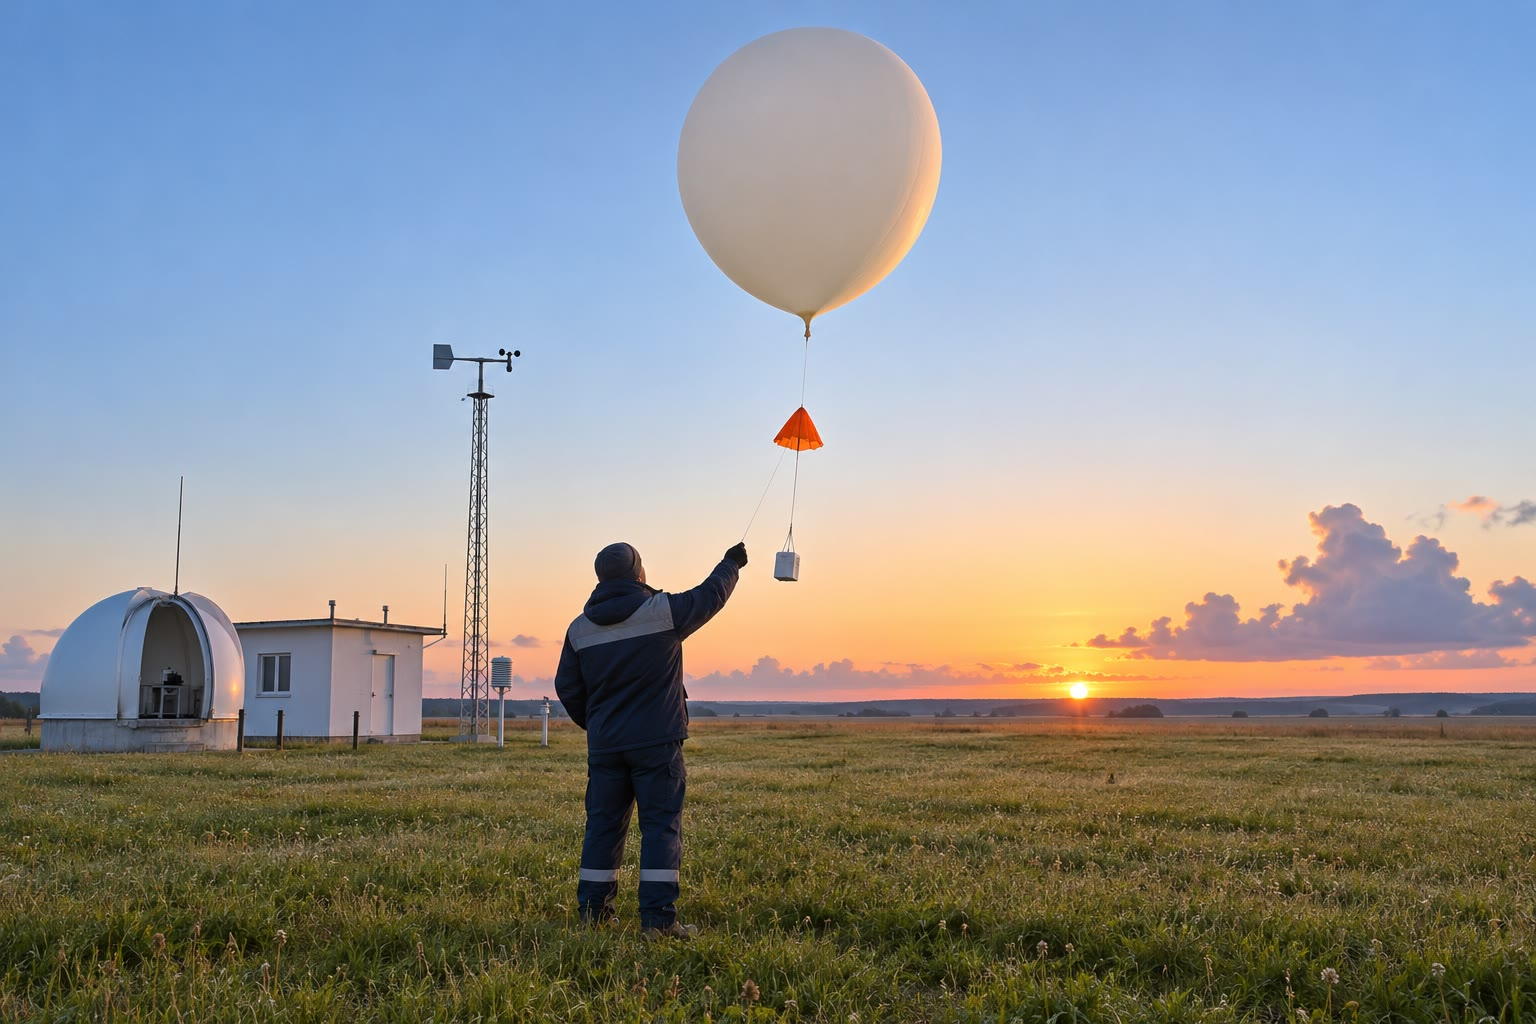
\includegraphics[width=\linewidth]{images/book4/ai/b2-radiosonde-launch.jpg}

{\scriptsize Uma radiossonda lançada ao amanhecer de uma estação meteorológica (ilustração gerada
por IA).}
\end{minipage}
% ledger: nws:radiosonde, nws4:upperair
\end{inthefield}

\section*{Exercícios}\label{sec:b2:atmospheric-thermodynamics:exercises}

Dados para os exercícios, salvo indicação em contrário: $e_s(T) = \qty{6.117}{hPa} \times
\exp[\qty{5419}{K} \times (1/\qty{273.16}{K} - 1/T)]$; $\varepsilon = 0.622$, $R_d =
\qty{287.0}{J.kg^{-1}.K^{-1}}$, $R_v = \qty{461.5}{J.kg^{-1}.K^{-1}}$, $c_p =
\qty{1004.5}{J.kg^{-1}.K^{-1}}$, $L = \qty{2.501e6}{J/kg}$, $g = \qty{9.81}{m.s^{-2}}$,
$\Gamma_d = \qty{9.8}{K/km}$.
% ledger: nist4:water-sat, iapws4:sublimation, const:R, earth:Mmol, nist4:water-mw, nasa:grc-gamma

\begin{exercise}[$\star$]\label{exo:b2:atmospheric-thermodynamics:1}
A \qty{850}{hPa} a temperatura é \qty{10.0}{\celsius} e o ponto de orvalho \qty{5.0}{\celsius}.
(a) Calcule a \omterm{def:b2:atmospheric-thermodynamics:moist-air}{pressão de vapor} e a \omterm{def:b2:atmospheric-thermodynamics:moist-air}{pressão de vapor} de saturação. (b) Calcule a umidade relativa.
(c) Calcule a \omterm{def:b2:atmospheric-thermodynamics:moist-air}{razão de mistura} e a \omterm{def:b2:atmospheric-thermodynamics:moist-air}{umidade específica}, em gramas por quilograma.
\end{exercise}

\begin{exercise}[$\star$]\label{exo:b2:atmospheric-thermodynamics:2}
(a) Em quantos por cento por kelvin $e_s$ aumenta a \qty{0}{\celsius}, \qty{20}{\celsius} e
\qty{30}{\celsius}? (b) Calcule $e_s$ a \qty{20}{\celsius} e a \qty{25}{\celsius}, e sua
razão; compare com $1.063^5$. (c) O valor medido a \qty{20}{\celsius} é
\qty{23.39}{hPa}. Quanto a fórmula erra, e em que sentido? Por quê?
\end{exercise}
% ledger: nist4:water-sat

\begin{exercise}[$\star$]\label{exo:b2:atmospheric-thermodynamics:3}
Ao meio-dia o ar da superfície está a \qty{30}{\celsius} com um ponto de orvalho de \qty{14}{\celsius}. (a) A
que altura acima do solo se formam as bases dos cúmulos? (b) Qual é a temperatura de uma parcela
ali, pela adiabática seca? (c) Qual é seu ponto de orvalho ali, com $\Gamma_{\text{orv}} =
\qty{1.8}{K/km}$? Comente. (d) Mais tarde o ar aquece até \qty{33}{\celsius}, com o ponto de orvalho
inalterado. Onde ficam agora as bases das nuvens?
\end{exercise}

\begin{exercise}[$\star$]\label{exo:b2:atmospheric-thermodynamics:4}
Leia o diagrama skew-T da sondagem de Norman. (a) Até que pressão o ar junto ao
solo está saturado, ou quase? (b) Onde está a inversão, e como ela aparece? (c) Leia o
NCL, o NCE e o NE da parcela da superfície. (d) Como se comparam o ponto de orvalho e a temperatura
logo acima da inversão, e o que isso diz sobre esse ar?
\end{exercise}
% ledger: data:b4-sounding

\begin{exercise}[$\star\star$]\label{exo:b2:atmospheric-thermodynamics:5}
Um ar tropical a \qty{1000}{hPa} tem $T = \qty{30.0}{\celsius}$ e $r = \qty{20}{g/kg}$. (a) Calcule
sua \omterm{def:b2:atmospheric-thermodynamics:virtual}{temperatura virtual} exatamente e com a aproximação $T(1 + 0.61\,r)$. (b) Calcule as densidades
desse ar e do ar seco à mesma temperatura e pressão. (c) Quanto o ar seco teria de ser
aquecido para ficar tão leve? (d) Por que isso importa para a convecção sobre mares quentes?
\end{exercise}

\begin{exercise}[$\star\star$]\label{exo:b2:atmospheric-thermodynamics:6}
Use a \cref{prop:b2:atmospheric-thermodynamics:gamma-s} a \qty{1000}{hPa}, com $r_s$ da
\cref{prop:b2:atmospheric-thermodynamics:humidity}. (a) Calcule $r_s$ e $\Gamma_s$ a
\qty{0}{\celsius}, \qty{20}{\celsius} e \qty{30}{\celsius}. (b) Quanto mais quente que uma parcela
seca está uma parcela saturada a \qty{20}{\celsius} depois de subir \qty{1}{km}, se seu gradiente
continuar o mesmo? (c) Por que a diferença diminui mais acima?
\end{exercise}

\begin{exercise}[$\star\star$]\label{exo:b2:atmospheric-thermodynamics:7}
A parcela da superfície de Norman ($p = \qty{971.1}{hPa}$, $T = \qty{19.0}{\celsius}$, $T_d =
\qty{18.5}{\celsius}$) tem seu NCL a \qty{18.35}{\celsius}. (a) Calcule sua \omterm{def:b2:atmospheric-thermodynamics:moist-air}{razão de mistura}, sua
temperatura potencial e sua \omterm{def:b2:atmospheric-thermodynamics:theta-e}{temperatura potencial equivalente}. (b) Levantada, ela está a
\qty{-8.9}{\celsius} a \qty{500}{hPa}, saturada. Calcule ali seus $\theta$ e $\theta_e$.
(c) Qual dos dois se conserva?
\end{exercise}
% ledger: data:b4-sounding

\begin{exercise}[$\star\star$]\label{exo:b2:atmospheric-thermodynamics:8}
Uma parcela é mais quente que o ambiente em \qty{4}{K} entre \qty{700}{hPa}, seu NCE, e
\qty{300}{hPa}, seu NE; despreze a correção de \omterm{def:b2:atmospheric-thermodynamics:virtual}{temperatura virtual}. (a) Calcule sua CAPE. (b)
Calcule $w_{\max}$. (c) Em que classe cai a CAPE? (d) Num diagrama skew-T, que
forma tem a área positiva, e por que sua área é a que foi calculada?
\end{exercise}
% ledger: hgx:cape

\begin{exercise}[$\star\star$]\label{exo:b2:atmospheric-thermodynamics:9}
Tome $A = \qty{2.1}{nm}$ e o sulfato de amônio, $\kappa = 0.61$. (a) Calcule o diâmetro crítico
e a \omterm{def:b2:atmospheric-thermodynamics:microphysics}{supersaturação} crítica de uma partícula seca de \qty{80}{nm}. (b) Qual é a menor partícula seca
ativada num ar a \qty{0.3}{\percent} de \omterm{def:b2:atmospheric-thermodynamics:microphysics}{supersaturação}? E a \qty{0.1}{\percent}? (c) Uma corrente ascendente
eleva a \omterm{def:b2:atmospheric-thermodynamics:microphysics}{supersaturação} de \qty{0.1}{\percent} para \qty{0.3}{\percent}: o que acontece com o
número de gotículas, e com seu tamanho para a mesma água líquida?
\end{exercise}
% ledger: pk07:kappa, pk07:kohler

\begin{exercise}[$\star\star\star$]\label{exo:b2:atmospheric-thermodynamics:10}
A parcela da superfície de Norman tinha uma CIN de cerca de \qty{-130}{J/kg} com a \omterm{def:b2:atmospheric-thermodynamics:virtual}{temperatura virtual}.
(a) Com que velocidade vertical ela teria de deixar o solo para chegar a seu NCE por seu próprio
impulso? (b) O topo da inversão está a \qty{889.1}{hPa} e \qty{20.5}{\celsius}. Até que
temperatura o ar da superfície a \qty{971.1}{hPa} deve aquecer para que uma parcela levantada adiabaticamente
a seco não fique mais fria que o topo da inversão? (c) Se seu ponto de orvalho ficasse em
\qty{18.5}{\celsius}, onde ficaria a base de sua nuvem? (d) Cite duas maneiras pelas quais a atmosfera
remove uma tampa assim sem o sol.
\end{exercise}
% ledger: data:b4-sounding, nws4:cin

\begin{exercise}[$\star\star\star$]\label{exo:b2:atmospheric-thermodynamics:11}
(a) Mostre a partir da \cref{prop:b2:atmospheric-thermodynamics:gamma-s} que $\Gamma_s \to \Gamma_d$
quando $r_s \to 0$. (b) Mostre que, quando $Lr_s/(R_dT) \gg 1$, $\Gamma_s \to gR_vT/(LR_d)$, e
calcule-o a \qty{303}{K}. (c) Compare com o $\Gamma_{\text{orv}}$ da
\cref{prop:b2:atmospheric-thermodynamics:lcl} quando $T_d = T$, e explique por que os dois limites
coincidem. (d) O limite de (b) é atingido na atmosfera? Use o valor $\Gamma_s =
\qty{3.4}{K/km}$ a \qty{30}{\celsius} e \qty{1000}{hPa}.
\end{exercise}

\begin{exercise}[$\star\star\star$]\label{exo:b2:atmospheric-thermodynamics:12}
Sobre a água sobrerresfriada e sobre o gelo as \omterm{def:b2:atmospheric-thermodynamics:moist-air}{pressões de vapor} de saturação são 2.868 e
\qty{2.599}{hPa} a \qty{-10}{\celsius}, 1.257 e \qty{1.032}{hPa} a \qty{-20}{\celsius}.
(a) Calcule a \omterm{def:b2:atmospheric-thermodynamics:microphysics}{supersaturação} em relação ao gelo de um ar saturado em relação à água nas duas temperaturas. (b)
Compare com as \omterm{def:b2:atmospheric-thermodynamics:microphysics}{supersaturações} com que as gotículas se ativam. (c) Explique por que uma nuvem de
gotículas sobrerresfriadas que recebe alguns cristais de gelo se transforma em gelo. (d) Por que o efeito é
mais fraco perto de \qty{0}{\celsius}?
\end{exercise}
% ledger: iapws4:sublimation, su26:svp, nws4:ccn-bergeron

\begin{problem}[{Problema de fim de semana --- ler a sondagem da manhã}]\label{pb:b2:atmospheric-thermodynamics:1}
A tabela dá a sondagem das 12 UTC de Norman, Oklahoma, em 16 de abril de 2026, nos níveis usados
aqui: pressão, altitude acima do nível do mar, temperatura, ponto de orvalho, e a temperatura da
parcela da superfície levantada como no \cref{met:b2:atmospheric-thermodynamics:lift}, calculada
integrando a \cref{prop:b2:atmospheric-thermodynamics:gamma-s} em pequenos passos. A sondagem
indica a tropopausa a \qty{235.3}{hPa} e \qty{10954}{m}. Use os dados dos exercícios e
as temperaturas (não as temperaturas virtuais), salvo indicação em contrário.

\begin{center}
\small
\begin{tabular}{rrrrr}
\hline
$p$ (\unit{hPa}) & $z$ (\unit{m}) & $T$ (\unit{\celsius}) & $T_d$ (\unit{\celsius}) &
$T_{\text{parcel}}$ (\unit{\celsius}) \\
\hline
971.1 & 345 & 19.0 & 18.5 & 19.0 \\
925.0 & 763 & 17.3 & 17.3 & 16.9 \\
907.7 & 924 & 16.4 & 16.4 & 16.2 \\
889.1 & 1102 & 20.5 & 9.5 & 15.4 \\
850.0 & 1489 & 18.6 & $-1.8$ & 13.7 \\
700.0 & 3110 & 4.5 & $-12.2$ & 6.1 \\
500.0 & 5725 & $-18.4$ & $-36.6$ & $-8.9$ \\
400.0 & 7357 & $-30.4$ & $-55.6$ & $-20.4$ \\
300.0 & 9349 & $-42.7$ & $-66.3$ & $-37.1$ \\
250.0 & 10560 & $-49.8$ & $-69.8$ & $-48.3$ \\
200.0 & 12006 & $-52.3$ & $-78.3$ & $-61.8$ \\
\hline
\end{tabular}
\end{center}

\medskip\noindent\textbf{Parte I --- O ar junto ao solo.}
\begin{enumerate}
  \item Calcule a \omterm{def:b2:atmospheric-thermodynamics:moist-air}{pressão de vapor} do ar da superfície, com uma casa decimal.
  \item Calcule sua \omterm{def:b2:atmospheric-thermodynamics:moist-air}{razão de mistura}, com uma casa decimal.
  \item Calcule sua \omterm{def:b2:atmospheric-thermodynamics:moist-air}{umidade específica}.
  \item Calcule sua umidade relativa.
  \item Quanto sua \omterm{def:b2:atmospheric-thermodynamics:virtual}{temperatura virtual} excede sua temperatura?
  \item Calcule a altura de seu NCL acima do solo com a regra dos \qty{125}{m}, e a pressão
        ali (tome uma \omterm{def:b2:atmospheric-thermodynamics:virtual}{temperatura virtual} média de \qty{294.7}{K} para a camada).
  \item Calcule sua temperatura potencial.
\end{enumerate}

\medskip\noindent\textbf{Parte II --- A tampa e as camadas acima.}
\begin{enumerate}[resume]
  \item A \qty{925}{hPa}, a parcela está mais quente ou mais fria que o ambiente, e quanto?
  \item Calcule o gradiente entre 907.7 e \qty{889.1}{hPa}. Que tipo de camada é essa?
  \item Quanto a parcela está mais fria que o ambiente a \qty{889.1}{hPa}?
  \item Calcule a umidade relativa a \qty{850}{hPa}. De onde poderia ter vindo esse ar?
  \item Calcule o gradiente médio entre 850 e \qty{500}{hPa} e classifique a camada.
  \item Calcule o índice de levantamento e sua classe.
\end{enumerate}

\medskip\noindent\textbf{Parte III --- A energia.}
\begin{enumerate}[resume]
  \item Calcule o excesso $\Delta T = T_{\text{parcela}} - T$ em cada nível da tabela.
  \item Encontre o NCE interpolando $\Delta T$ linearmente em $\ln p$, com aproximação de um hectopascal,
        e sua altitude interpolando $z$ da mesma maneira.
  \item Encontre o NE e sua altitude da mesma maneira. Compare com a tropopausa.
  \item Calcule a CAPE pela regra dos trapézios em $\ln p$, do NCE ao NE passando pelos
        níveis da tabela.
  \item Em que classe ela cai?
  \item Calcule a CIN da mesma maneira, do solo até o NCE.
  \item Um cálculo numa grade de \qty{1}{hPa} dá uma CAPE de \qty{2100}{J/kg} com as
        temperaturas e \qty{2230}{J/kg} com as temperaturas virtuais. Por que os três valores
        diferem?
\end{enumerate}

\medskip\noindent\textbf{Parte IV --- A tempestade que o ar poderia alimentar.}
\begin{enumerate}[resume]
  \item Que velocidade vertical dá a teoria da parcela com a CAPE da questão 17?
  \item À metade dessa velocidade o tempo todo, quanto tempo o ar levaria para subir do NCE ao NE?
  \item Cite dois efeitos que tornam mais lenta uma corrente ascendente real.
  \item Em resumo: que velocidade de corrente ascendente a teoria da parcela prevê para uma tempestade alimentada pelo
        ar da superfície desta manhã?
\end{enumerate}
\end{problem}
% ledger: data:b4-sounding, hgx:cape, nws4:lifted-index, nws4:cape
